% autosam.tex
% Annotated sample file for the preparation of LaTeX files
% for the final versions of papers submitted to or accepted for 
% publication in AUTOMATICA.

% See also the Information for Authors.

% Make sure that the zip file that you send contains all the 
% files, including the files for the figures and the bib file.

% Output produced with the elsart style file does not imitate the
% AUTOMATICA style. The style file is generic for all Elsevier
% journals and the output is laid out for easy copy editing. The
% final document is produced from the source file in the
% AUTOMATICA style at Elsevier.

% You may use the style file autart.cls to obtain a two-column 
% document (see below) that more or less imitates the printed 
% Automatica style. This may helpful to improve the formatting 
% of the equations, tables and figures, and also serves to check 
% whether the paper satisfies the length requirements.

% Please note: Authors must not create their own macros.

% For further information regarding the preparation of LaTeX files 
% for Elsevier, please refer to the "Full Instructions to Authors" 
% from Elsevier's anonymous ftp server on ftp.elsevier.nl in the
% directory pub/styles, or from the internet (CTAN sites) on
% ftp.shsu.edu, ftp.dante.de and ftp.tex.ac.uk in the directory
% tex-archive/macros/latex/contrib/supported/elsevier.


%\documentclass{elsart}               % The use of LaTeX2e is preferred.

\documentclass[twocolumn]{autart}    % Enable this line and disable the 
                                     % preceding line to obtain a two-column 
                                     % document whose style resembles the
                                     % printed Automatica style.


\usepackage{graphicx}          % Include this line if your 
                               % document contains figures,
%\usepackage[dvips]{epsfig}    % or this line, depending on which
                               % you prefer.

% User imported packages
\usepackage{amsmath}
\usepackage{amsfonts}
\usepackage{algorithm}
\usepackage{algpseudocode}
\usepackage{tikz}
\usepackage{environ}
\usepackage{layouts}



\makeatletter
\newsavebox{\measure@tikzpicture}
\NewEnviron{scaletikzpicturetowidth}[1]{%
  \def\tikz@width{#1}%
  \def\tikzscale{1}\begin{lrbox}{\measure@tikzpicture}%
  \BODY
  \end{lrbox}%
  \pgfmathparse{#1/\wd\measure@tikzpicture}%
  \edef\tikzscale{\pgfmathresult}%
  \BODY
}
\makeatother

\begin{document}

\begin{frontmatter}
% Running title for regular 
% papers but only if the title  
% is over 5 words. Running title 
% is not shown in output.
%\runtitle{Insert a suggested running title}

\title{Localisation and Sensor Privacy Using the Extended Information Filter and Secure Weighted Aggregation\thanksref{footnoteinfo}} % Title, preferably not more than 10 words.

\thanks[footnoteinfo]{This paper was not presented at any IFAC 
meeting. Corresponding author Uwe~D.~Hanebeck. Tel. +49--721--608--43909.}

% Add the 
% e-mail address 
% (ead) as shown
\author[ISAS]{Marko Ristic}\ead{marko.ristic@kit.edu},
\author[ISAS]{Benjamin Noack}\ead{noack@kit.edu},
\author[ISAS]{Uwe D. Hanebeck}\ead{uwe.hanebeck@kit.edu}

\address[ISAS]{Intelligent Sensor-Actuator-Systems Laboratory, Institute for Anthropomatics, Karlsruhe Institute of Technology, 76131 Karlsruhe, Germany}  % Please supply

% Five to ten keywords,  
% chosen from the IFAC 
% keyword list or with the 
% help of the Automatica 
% keyword wizard
\begin{keyword}
System state estimation; Data privacy; Sensor fusion; Kalman filters.
\end{keyword}


\begin{abstract} % Abstract of not more than 200 words.
Distributed state estimation and localisation methods have become increasingly popular with the rise of ubiquitous computing, and have led naturally to an increased concern regarding data and estimation privacy. Traditional distributed sensor navigation methods involve the leakage of sensor information or navigator location during localisation protocols and fail to preserve participants’ data privacy. Existing approaches which provide such guarantees, fail to address sensor and navigator privacy in some common model-based non-linear measurement localisation methods forfeiting broad applicability. We define a cryptographically secure weighted aggregation scheme which we apply to the Extended Kalman Filter with range-sensor measurements, and show that navigator location, sensor locations and sensor measurements can remain private during navigation. The security requirements, leakage, and cryptographic proof are given for the private filter and weighted aggregation scheme, and simulations of the filter are used to evaluate the accuracy and performance of the method. Our approach defines a novel, computationally plausible and cryptographically private, model-based localisation filter with direct application to environments where nodes may not be fully trusted and data is considered sensitive.
\end{abstract}

\end{frontmatter}

\section{Introduction}


--

Introduce localisation, filtering and the need for privacy. 

Examples of environments where privacy is relevant and concrete examples where lack of privacy could have large costs

Methods for introducing security and privacy include differential privacy methods and encryption methods. 

Differential privacy involves using statistical noise as security to make individual users' information cannot be deduced. Often requires a trusted aggregator, although secure aggregation methods exist. always requires noising result such that the outcome is not exact (a problem in localisation).

Encryption schemes involve formal indistinguishability proofs typically over bits or integers. They rely on computationally hard problems involving security parameters of a sufficiently large size; therefore the additional computational requirements of using encryption schemes should be pointed out and what this means in a real-time distributed sensor system. Continuing, explain public-key cryptography applicability to distributed systems; difference to symmetric schemes. Homomorphic encryption power and use case. Why FHE isn't used often, why additive partially homomorphic encryption is.

Advancements in function providing encryption schemes such as homomorphic encryption have also led to several other types of schemes which have found uses in signal processing. Private aggregation schemes allow the secure computation of the sum of encrypted values originating from different parties, leaking only the final result. When considering such multi-party encryption protocols, formal security definitions must now also incorporate the added dangers of colluding malicious parties, and lead to new notions of security. For example Aggregator Obliviousness (AO) is typically proven for private aggregation schemes, while alternatives such as Private Weighted Secure Aggregator Obliviousness (pWSAO) exist for other specific use-cases.

Another example of function providing encryption, and a generalisation of private aggregation, is called functional encryption (FE) and its distributed extension, multi-client functional encryption (MCFE), which allow the unencrypted result of an arbitrary function to be computed from encrypted inputs. General FE and MCFE are known to be quite computationally expensive (from meeting with ITI and student Johannes - need ref.) but alternatives providing only a subset of possibly computable function exist; for example, inner product encryption.

Several of the aforementioned encryption schemes have found uses in secure localisation, estimation, and control.

\subsection{Relevant Literature on Encrypted Localisation and Estimation}

Model-free localisation using homomorphic encryption examples include polygon thing, WSN examples which protect against adversaries but in the case of the WSN paper. don't preserve anchor privacy. Importantly, model-based filtering and localisation provide more accurate estimates and these are not applicable there.

Model-based estimation examples include Aristov paper (which requires a linear model, and a hierarchy of sensors), Farokhi paper (which requires the controller compute entirely in encrypted space and send input back to actuator - supporting only the cloud-as-a-service type architectures) and Alexandru paper (which implements a distributed control environment but requires a constant gain matrix K)

pWSAO achieved in Alexandru weighted aggregation, but requires redistributing keys at every timestep resulting in a costly operation, and a complicated communication protocol.

In addition to applying suitable encryption schemes to signal processing tasks, care must be taken when converting sensor output into an encryptable homomorphic format. As is the case with our proposed localisation method, real number sensor output does not trivially encode to integers such that the homomorphic properties provided by an additive encryption scheme over integers keep the underlying real numbers consistent. Methods for handling the encoding of real numbers such that they can be used in homomorphic encryption exist. Google bignum adds power but risks overflow and leaks exponents, Farokhi leaks no information but allows only a single multiplication (extendable to more but each further multiplication limits the real number size and increases the risk of overflow).

Briefly describe navigator scenario and our contributions

Section Summary
%In Section \ref{sec:private_localisation} we will show how this scheme can be used to compute the measurement covariance and measurement vector homomorphically at each sensor, and allow the navigator to update their 

\subsection{Notation}
Notation


\section{Problem Statement} \label{sec:problem_statement}

Restate the scenario but more formally. Give a concrete example - plane and signal towers.

Exact security guarantees we aim for, as well as the definitions for these guarantees (pWSAO and indistinguishability but in context of localisation as well). Note that learning only the sum in aggregation (as is normal in AO) would, in this case, tell the navigator the average location and measurements of all sensors, which is fine as it does not disclose any exact sensor.

Passive attacks only from sensors to learn navigator position (Otherwise one could do some kind of attack that would send a fake measurement and note the change in its own measurements - possible this would give away the average of other sensors' measurements but unclear). Any largely incorrect inputs from sensors may also be detectable by comparison to alternative navigator onboard sensors (GPS etc.). Justify by saying sensors need to behave for localisation to work in the first place.

Active attacks from navigator to find sensor location allowed, but assume that weights sent to all sensors are the same. In a wireless setting, all sensors would receive all broadcast weights anyway. While special hardware, which may support directional broadcasting or receiving, could be used to locate sensors individually this is beyond the scope of what is considered in our problem.

Point out that learning the aggregation of sensor outputs, which contains measurement and location information also means that the average location and measurement of the sensors may be leaked, and is accepted as a part of the leakage as it is inferrable from the aggregation scheme and any functioning model-based localisation where measurements are not known

Rough computational capabilities expected by parties

Fixed sensor subsets of which only whole subsets can be used at once. Maybe a picture of what this might look like in a high level distributed localisation diagram. Should consider that this sub-grouping would also mean the leakage of the average sensor/measurement of each subset not all sensors at once. This should be considered when choosing sensor subsets and locations.




\section{Privacy-Preserving Weighted Aggregation}
For achieveing the goal of private localisation defined in Section \ref{sec:problem_statement} we require a cryptographic scheme which allows a time-series of homomorphically computed linear combinations of encrypted weights, to be summed by a privacy-preserving aggregation scheme. In our case, weights $\omega_1, \dots , \omega_m$ are encrypted and broadcast by the navigator, linear combinations $\sum^m_{j=1}x_{j,i}^{(t)}\omega_i$ are computed by the sensors $i \in \{1, \dots ,n\}$ at time $t$, and aggregation is computed back at the navigator. This has been summarized in Figure \ref{fig:agg_steps}. In Section \ref{sec:private_localisation} we will show how this scheme can be used to compute measurement covariances and measurement vectors homomorphically, and update the Extended Information Filter while preserving privacy. 

\begin{figure}[htbp]
\centering
\vspace{\baselineskip}
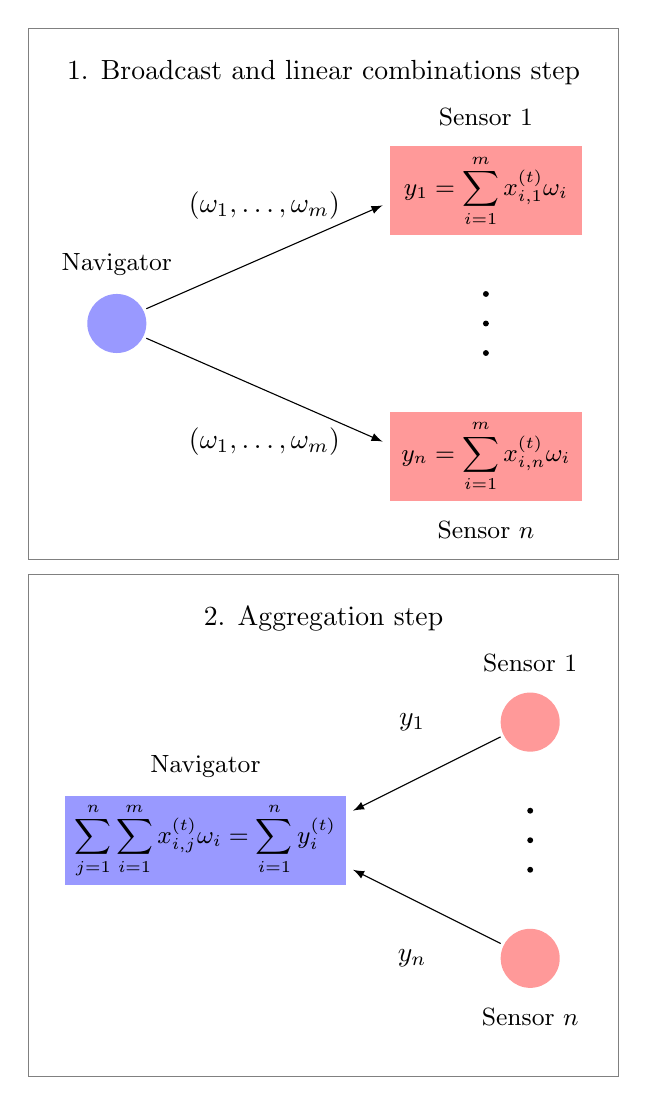
\begin{tikzpicture}[scale=0.75]
    % Step 1
    \node at (5,22.5) {1. Broadcast and linear combinations step};
    % Navigator
    \node at (1.5,19.25) {\small Navigator};
    \fill (1.5,18.25) [blue!40] ellipse (0.5 and 0.5);
    % Sensors
    \node at (7.75,21.75) {\small Sensor $1$};
    \fill [red!40] (6.125,19.75) rectangle (9.375,21.25);
    \node at (7.75,20.5) {\small $\displaystyle y_1 = \sum^m_{i=1}x_{i,1}^{(t)}\omega_i$};
    \node at (7.75,14.75) {\small Sensor $n$};
    \fill [red!40] (6.125,15.25) rectangle (9.375,16.75);
    \node at (7.75,16) {\small $\displaystyle y_n = \sum^m_{i=1}x_{i,n}^{(t)}\omega_i$};
    \fill [black] (7.75,18.75) circle (0.05);
    \fill [black] (7.75,17.75) circle (0.05);
    \fill [black] (7.75,18.25) circle (0.05);
    % Lines
    \draw [-latex] plot[smooth, tension=.7] coordinates {(2,18.5) (6,20.25)};
    \draw [-latex] plot[smooth, tension=.7] coordinates {(2,18) (6,16.25)};
    \node at (4,20.25) {$(\omega_1,\dots ,\omega_m)$};
    \node at (4,16.25) {$(\omega_1,\dots ,\omega_m)$};
    
    % Step 2
    \node at (5,13.25) {2. Aggregation step};
    % Navigator
    \node at (3,10.75) {\small Navigator};
    \fill [blue!40] (0.625,8.75) rectangle (5.375,10.25);
    \node at (3,9.5) {\small $\displaystyle \sum^{n}_{j=1}\sum^{m}_{i=1} x_{i,j}^{(t)}\omega_i = \sum^n_{i=1}y^{(t)}_{i}$};
    % Sensors
    \node at (8.5,12.5) {\small Sensor $1$};
    \fill  (8.5,7.5) [red!40] ellipse (0.5 and 0.5);
    \node at (8.5,6.5) {\small Sensor $n$};
    \fill  (8.5,11.5) [red!40] ellipse (0.5 and 0.5);
    \fill [black] (8.5,10) circle (0.05);
    \fill [black] (8.5,9) circle (0.05);
    \fill [black] (8.5,9.5) circle (0.05);
    % Lines
    \draw [-latex] plot[smooth, tension=.7] coordinates {(8,11.25) (5.5,10)};
    \draw [-latex] plot[smooth, tension=.7] coordinates {(8,7.75) (5.5,9)};
    \node at (6.5,11.5) {$y_1$};
    \node at (6.5,7.5) {$y_n$};
    
    % Bounding rectangles
    \draw [gray] (0,23.25) rectangle (10,14.25);
    \draw [gray] (0,14) rectangle (10,5.5);
\end{tikzpicture}
\vspace{\baselineskip}
\caption{Required weighted aggregation scheme}
\label{fig:agg_steps}
\end{figure}

The security of a cryptographic scheme is typically defined by a security \textit{game}, which captures both the desired privacy guarantees, as well as the capabilities of attackers \cite{katzIntroductionModernCryptography2008}. Before defining the desired security of our scheme, we note that it has properties of both an additive homomorphic encryption scheme, and a privacy-preserving aggregation scheme. The typical security requirement for a homomorphic encryption scheme is Indistinguishability under the Chosen Plaintext Attack model (IND-CPA) \cite{}. Informally, IND-CPA states that an attacker who can choose plaintext messages to be encrypted at will, gains no additional information about an unkonwn plaintext message when they learn only its encryption. The more formal security game for IND-CPA has been given in Appendix \ref{app:ind-cpa}. Privacy-preserving aggregation, without weights, aims for the security goal of Aggregator Obliviousness (AO) \cite{}. AO states that no colluding subset of participants gains any additional information about the aggregation values from the remaining parties, given only their encryption, with the exception of learning only their sum if the aggregator is among the colluding subset. The game for AO has been given in Appendix \ref{app:ao}.

Our desired weighted aggregation method has two security goals. Firstly, that encrypted values are indistinguishable from random to sensors, and secondly, that individual weighted values remain unknown to the navigator, who learns only the final weighted sum. From the definitions above, it is clear that an IND-CPA secure encryption of navigator produced weights is sufficient for the first goal, while the definition of AO needs to be altered to incooporate weights for the second.

Such an altered aggregation games has been defined in \cite{alexandruEncryptedCooperativeControl2019} as private Weighted Sum Aggregator Obliviousness (pWSAO). In overview, the game states that given given weights --- not the case, need to define our own slightly different version (but we get to name it something else at least)

and is defined as follows




Our weighted aggregation method relies on the decisional composite residuosity assumption (DCRA) originally defined by Paillier in \cite{paillierPublicKeyCryptosystemsBased1999}. The aggregation method can be seen as a combination of the additive homomorphic Paillier encryption scheme, which additionally allows multiplication of an encrypted message with a plaintext value, and the Joye-Libert private stream-aggregation scheme. Both of these schemes base their security on the DCRA, and their descriptions are given briefly below before defining our weighted aggregation scheme.


% A number $z$ is said to be an $n$th residue modulo $n^2$ if there exists a number $y \in \mathbb{Z}^{*}_{n^2}$ such that
% \begin{equation}
%     z = y^n \pmod{n^2},
% \end{equation}
% where $n=pq$ is the product of two large primes. DCRA states that distinguishing an $n$th residue modulo $n^2$ from non $n$th residues is a hard problem, and is shown to be a reduction of the 

\subsection{Paillier Encryption Scheme}
The Paillier encryption scheme is an additively homomorphic encryption scheme which functions over a finite group $\mathbb{G}$, containing 

% TODO not true I think - just keep it simple instead - a subgroup where the DCRA holds and is of an unknown order, and another subgroup where discrete logarithms are easily computable.

Key generation of the Paillier scheme is performed by choosing two sufficiently large primes $p$ and $q$, and computing $n=pq$. A generator $g$ is also required for encryption, which is often set to $g=n+1$ when $p$ and $q$ are of equal bit length \cite{}. The public key is then given by $(n, g)$ and secret key by $(p, q)$.

Encryption of a plaintext message $m \in \mathbb{Z}_n$, producing ciphertext $c \in \mathbb{Z}^{*}_{n^2}$, is computed by
\begin{equation}
    c = g^m r^n \pmod{n^2}
\end{equation}
for a randomly chosen $r \in \mathbb{Z}_{n}$. The $r^n$ term can be considered as the noise which hides the value $g^m \pmod{n^2}$, which due to the scheme construction, is an easily computable discrete logarithm. The decryption of a ciphertext is computed by
\begin{equation}
    m = \frac{L(c^\lambda\pmod{n^2})}{L(g^\lambda\pmod{n^2})} \pmod{n}
\end{equation}
where $\lambda = \operatorfont{lcm}(p-1, q-1)$ and $L(u) = \frac{u-1}{n}$.

In addition to encryption and decryption, the following homomorphic functions are provided by the Paillier scheme. $\forall m_1,m_2 \in \mathbb{Z}_n$,
\begin{align}
    \mathcal{D}(\mathcal{E}(m_1)\mathcal{E}(m_2)\!\pmod{n^2}) &= m_1+m_2\!\pmod{n} \\
    \mathcal{D}(\mathcal{E}(m_1)g^{m_2}\!\pmod{n^2}) &= m_1+m_2\!\pmod{n} \\
    \mathcal{D}(\mathcal{E}(m_1)^{m_2}\!\pmod{n^2}) &= m_1m_2\!\pmod{n}\,.
\end{align}

The scheme is shown to be indistinguishable under the chosen plaintext attack model (IND-CPA), which is considered the strongest form of security acheivable by a homomorphic encryption scheme \cite{}.

\subsection{Joye-Libert Privacy-Preserving Aggregation}
The Joye-Libert private stream aggregation scheme allows, at each time-step, encrypted time-series values originating from $N$ different measuring parties, to be summed up and decrypted by an aggregator. Time-series values are encrypted by their measuring party's private encryption key, and decrypted by the aggregator using its private key. The scheme functions over the same finite group $\mathbb{G}$ as the Paillier encryption scheme above.

A notable difference in key-generation for the aggregation scheme from a public-key scheme such as Paillier's scheme, is the requirement of an offline generation and distribution step by some trusted party. Similar to the Paillier scheme, key generation first requires choosing two sufficiently large, equal length, primes $p$ and $q$ and computing $n=pq$. In addition to $n$, a hash function $H:\mathbb{Z} \rightarrow \mathbb{Z}_{n^2}$ is defined, and the public key is set to $(n, H)$. The private keys are generated by choosing $N$ keys $sk_i,\,i \in \{1,\dots,N\}$ uniformly from $\mathbb{Z}_{n^2}$ and distributing them to all measuring parties, while the last key is set to
\begin{equation}
    sk_0 = -\sum^{N}_{i=1}sk_i \pmod{n^2}\,,
\end{equation}
and sent to the aggregator.

Encryption of plaintext $m_{i,t} \in \mathbb{Z}_n$ to ciphertext $c_{i,t} \in \mathbb{Z}_{n^2}$ at time $t$ is computed by participant $i$ as
\begin{equation}
    c_{i,t} = (n+1)^{m_{i,t}} H(t)^{sk_i} \pmod{n^2}\,,
\end{equation}
As with the interpretation of the noise term in the Paillier scheme, here $H(t)^{sk_i}$ can be seen as noise which hides the easily computable discrete logarithm $g^{m_{i,t}} \pmod{n^2}$, where $g=n+1$.

When all encryptions $c_{i,t},\,i \in \{1,\dots,N\}$ are sent to the aggregator, private summation and decryption are computed by the functions
\begin{equation}
    c_{t} = H(t)^{sk_0}\prod^{N}_{i=1}c_{i,t} \pmod{n^2}
\end{equation}
and
\begin{equation}
    \sum^{N}_{i=1}m_{i,t} = \frac{c_{t}-1}{n}\,. \label{eqn:agg_decryption}
\end{equation}
Correctness follows from $\sum^{N}_{i=0}sk_i = 0$, and therefore
\begin{align}
    &H(t)^{sk_0}\prod^{N}_{i=1}c_{i,t} \pmod{n^2} \\
    \equiv &H(t)^{sk_0}\prod^{N}_{i=1}(n+1)^{m_{i,t}} H(t)^{sk_i} \pmod{n^2} \\
    \equiv &H(t)^{\sum^N_{j=0}sk_j} \prod^{N}_{i=1}g^{m_{i,t}} \pmod{n^2} \\
    \equiv &(n+1)^{\sum^N_{i=1}m_{i,t}} \pmod{n^2}
\end{align}
which results in a solvable discrete logarithm by using \eqref{eqn:agg_decryption}, as defined in \cite{joyeScalableSchemePrivacyPreserving2013}, with no more noise term.

The aggregation scheme is proven to achieve aggregator obliviousness (AO), which in that no corrupted colluding subset learns anything about the individual messages of the non-corrupted participants, other than the final sum of messages if the aggregator is corrupted, and is proven in the random oracle model.

% Maybe rename this to Our Scheme or something like that
\section{Our Scheme}
Explain it in as an overview

% \begin{algorithm}
%     \caption{Paillier Key Generation}\label{paillier_key_gen}
%     \begin{algorithmic}[1]
%         \Procedure{PaillierKeyGen}{$security\_param$}
%         \State $p,q \gets$ \Call{GeneratePrimes}{$security\_param$}
%         \State $\lambda \gets$ \Call{lcm}{p,q}
%         \State $pk \gets (n, n+1)$
%         \State $sk \gets \lambda$
%         \State \Return $(pk, sk)$
%         \EndProcedure
%     \end{algorithmic}
% \end{algorithm}

\subsection{Proof}
Give the reduction proof here for pWSAO and implicit indistinguishability of weights. Alternatively, sketch it out here and give reduction proof in the appendix.


\section{Private Localisation}

\subsection{Integer Encoding for Real Numbers}

\subsection{Extended Information Filter}


\section{Private Localisation with Privacy-Preserving Sensors} \label{sec:private_localisation}
Explain it in as an overview. How is the aggregation scheme used, what does this require from the measurement model, why can this be a problem for normal distance sensors?

Explain how leakage of the final aggregation sum to the navigator means leakage of the average sensor location and measurement to the navigator. This is the reason for the acceptance of this leakage, as we pointed out in the problem statement section.

\subsection{Requirements for Measurement Model}

\subsection{Localisation Measurement Modification}
Show here the weighted integrals that give mean and variance of the new noise. If wanting to show more working, do this in the appendix section, but probably not needed.

Point out here that the further away the sensor is when it makes its distance measurement (the larger the measurement) the more Gaussian the noise and the better the filter. Give flight navigation as an applicable example with typically high distances.

Additionally increased range accuracy may be possible when sensors know the process model of the navigator, allowing them to run their own filter (more accurate than only measurements but not as accurate as the navigator's estimate from multiple sensors) and use their filtered estimated distance as the scaling factor when computing the modified measurement variance.

\subsection{Expanding Aggregation for Multi-dimensional Inputs}
Give 1D example that's intuitive (with $a^2b$) and then reduce the equivalent ND case ($A^\top BA$) to a set of weighted sums.

Ensure that timestamps are concatenated with the position so that no aggregation values are blinded by the same noise.

% Maybe name the scheme? That would be in the heading here
\subsection{Algorithm}
Piece together the whole algorithm here.
Give the algorithm as pseudocode (including encoding and encryption)


\section{Results}
Decide on what kind of simulations and which plots to make. run times would be nice this time around

Time results can be captured in one graph. Y-axis is time, X-axis is the number of sensors, each line (different colour) will show how the runtime changes as sensors are increased for different Paillier bit-sizes (at least 3: 512, 1024, 2048). Every data point should be the average over some X number of simulations.

Accuracy plots will describe error due to encoding and the average distance of the sensors to the navigator. All plots will use the same ground truth and initial state and covariance estimates (this way average error at each timestep from multiple runs makes sense).

Plot 1 will plot the RMSE of the average of X runs at each encoding size. A fixed layout of 4 mediumly spaced sensor will be used, and a fixed Paillier bit size.

Plot 2 will plot the RMSE as the average distance of sensors changes. Fixed encoding and Paillier bit size. Vary between 4 layouts where 4 sensors are either very close to the centre (and ground truth, and progressively further out)

Plot 3 will accompany plot 3 and display the 4 layouts (arrow for ground truth and points for the sensors).

A well-defined example.

\section{Conclusion}
Possible future work to consider writing here:
Hardware implementations, measurement handling which preservers Gaussian noise, or non-Gaussian noise methods, ways of sending less information form the navigator to the sensors at each time step, active sensor attacker model, different state encryptions received at sensors.

%---Rest is template---


% \section{Introduction}
% Video, patres conscripti, in me omnium vestrum ora atque oculos esse 
% conversos, video vos non solunn de vestro ac rei publicae, verum 
% etiam, si id depulsum sit, de meo periculo esse sollicitos. Est mihi 
% iucunda in malis et grata in dolore vestra erga me voluntas, sed eam, 
% per deos inmortales, deponite atque obliti salutis meae de vobis ac 
% de vestris liberis cogitate. Mihi si haec condicio consulatus data 
% est, ut omnis acerbitates, onunis dolores cruciatusque perferrem, 
% feram non solum fortiter, verum etiam lubenter, dum modo meis 
% laboribus vobis populoque Romano dignitas salusque pariatur.

% \begin{figure}
% \begin{center}
% 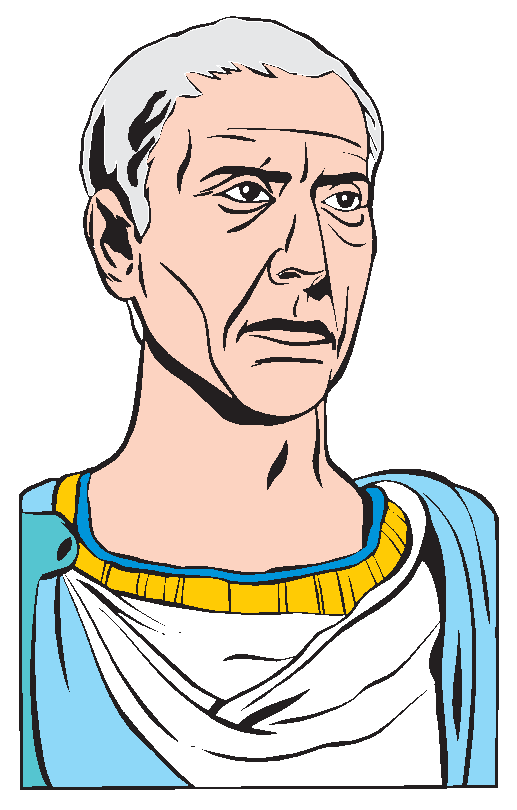
\includegraphics[height=4cm]{jcaesar.eps}    % The printed column  
% \caption{Gaius Julius Caesar, 100--44 B.C.}  % width is 8.4 cm.
% \label{fig1}                                 % Size the figures 
% \end{center}                                 % accordingly.
% \end{figure}

% % OR

% %\begin{figure}
% %\begin{center}
% %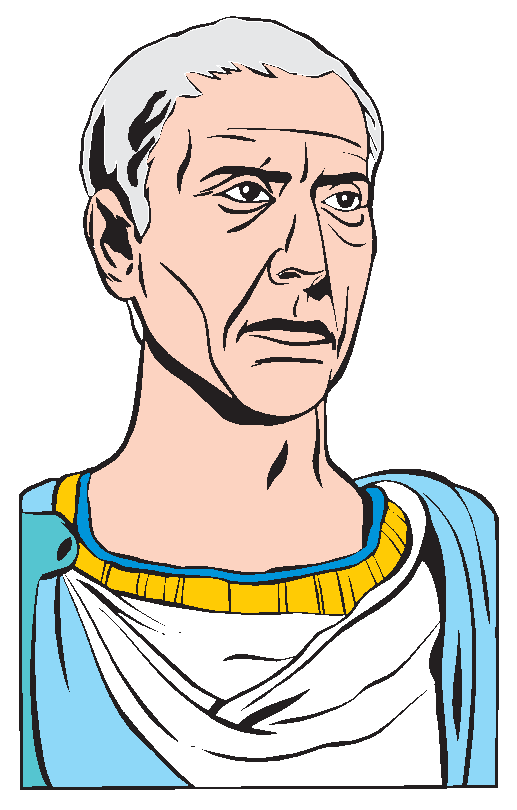
\epsfig{file=jcaesar,width=7cm}
% %\caption{Gaius Julius Caesar, 100--44 B.C.}
% %\label{fig1}
% %\end{center}
% %\end{figure}


% \subsection{A subsection}
% Marcus Tullius Cicero, 106--43 B.C. was a Roman statesman, orator, 
% and philosopher.  A major figure in the last years of the Republic, 
% he is best known for his orations against Catiline\footnote{
% This footnote should be very brief.}
% and for his mastery of Latin prose \cite{Heritage:92}. He was a 
% contemporary of Julius Caesar (Fig.~\ref{fig1}).

% \section{The argument}
% Some words might be appropriate describing equation~(\ref{e1}), if 
% we had but time and space enough.
% \begin{equation} \label{e1}
% {{\partial F}\over {\partial t}} =
% D{{\partial^2 F}\over {\partial x^2}}.
% \end{equation}
% See \cite{Abl:56}, \cite{AbTaRu:54}, \cite{Keo:58} and 
% \cite{Pow:85}.
% This equation goes far beyond the celebrated theorem ascribed to the great
% Pythagoras by his followers.
% \begin{thm}
% The square of the length of the hypotenuse of a right triangle equals the sum of the squares 
% of the lengths of the other two sides.
% \end{thm}
% \section{Epilogue}
% A word or two to conclude, and this even includes some inline 
% maths:  $R(x,t)\sim t^{-\beta}g(x/t^\alpha)\exp(-|x|/t^\alpha)$.

\begin{ack}                               % Place acknowledgements
Partially supported by the Roman Senate.  % here.
\end{ack}

\bibliographystyle{plain}        % Include this if you use bibtex 
                                 % and a bib file to produce the 
                                 % bibliography (preferred). The
                                 % correct style is generated by
                                 % Elsevier at the time of printing.
\bibliography{BibTeX/PrivateEIFLocalisation}

%\begin{thebibliography}{99}     % Otherwise use the  
                                 % thebibliography environment.
                                 % Insert the full references here.
                                 % See a recent issue of Automatica 
                                 % for the style.
%  \bibitem[Heritage, 1992]{Heritage:92}
%     (1992) {\it The American Heritage. 
%     Dictionary of the American Language.}
%     Houghton Mifflin Company.
%  \bibitem[Able, 1956]{Abl:56}
%     B.~C.~Able (1956). Nucleic acid content of macroscope. 
%     {\it Nature 2}, 7--9. 
%  \bibitem[Able {\em et al.}, 1954]{AbTaRu:54}   
%     B.~C. Able, R.~A. Tagg, and M.~Rush (1954).
%     Enzyme-catalyzed cellular transanimations.
%     In A.~F.~Round, editor, 
%     {\it Advances in Enzymology Vol. 2} (125--247). 
%     New York, Academic Press.
%  \bibitem[R.~Keohane, 1958]{Keo:58}
%     R.~Keohane (1958).
%     {\it Power and Interdependence: 
%     World Politics in Transition.}
%     Boston, Little, Brown \& Co.
%  \bibitem[Powers, 1985]{Pow:85}
%     T.~Powers (1985).
%     Is there a way out?
%     {\it Harpers, June 1985}, 35--47.

%\end{thebibliography}

% Each appendix must have a short title.
% Sections and subsections are supported
% in the appendices.
\appendix
\section{Indistinguishability under the Chosen Plaintext Attack (IND-CPA)} \label{app:ind-cpa}
\section{Aggregator Obliviousness (AO)} \label{app:ao}

\end{document}